\documentclass[
  aspectratio=169,
  draft=false,
  spanish,
]{beamer}

% ====================================
% Packages & Style
% ====================================

\usepackage{Personal}
\usetheme{Madrid}

% ====================================
% Portada
% ====================================

\title{Cálculo de Geodésicas en el Disco de Poincaré}
\author{Ángel Peñaflor}

% ====================================
% Documento
% ====================================

\begin{document}
\maketitle

\chapter{Introducción}
La geometría diferencial tiene como objetivo el estudio de las propiedades geométricas de las curvas y superficies a través del uso del cálculo diferencial e integral. Esta rama de las matemáticas tiene formalmente sus orígenes en siglo XIX, con las investigaciones realizadas por matemáticos como Carl Friedrich Gauss, Bernhard Riemann y Nikolái Lobachevsky sobre las propiedades de las superficies con curvatura. 

Si bien en sus inicios la geometría diferencial fue estudiada desde un punto de vista extrínseco, considerando a las curvas y superficies como partes de algún espacio ambiente más grande, heredando de manera natural propiedades de estos espacios, resultados como el \textit{theorema egregium} de Gauss resaltaron la importancia de las propiedades intrínsecas a las curvas y superficies, como lo son la longitud de una curva o la curvatura de una superficie.

Desde entonces ha habido grandes avances en esta área, los trabajos realizados durante el siglo XX por Henri Poincaré y Felix Hausdorff sobre los fundamentos formales de la topología dieron lugar a que matemáticos como Élie Cartan y Hassler Whitney replantaran la geometría diferencial en términos de lo que ahora conocemos como \textit{teoría de variedades}, la cual nos ha permitido generalizar las nociones de curva y superficies a dimensiones arbitrarias, librándonos además de la necesidad de tener que considerar a estos objetos como parte de un espacio ambiente más grande.

La teoría de variedades y la geometría diferencial han probado ser herramientas indispensables, no solo para las matemáticas, siendo de gran utilidad en el estudio de la topología, el análisis complejo, la geometría algebraica; sino también para la física, dando el marco matemático bajo el cual se entienden teorías como la relatividad general de Einstein o la teoría de gauge.

El presente trabajo está divido en tres capítulos.

El primer capítulo, titulado \textit{Variedades y mapas}, tiene como objetivo presentar definiciones y ejemplos básicos que permitan familiarizarnos con los objetos con los que estamos trabajando, las variedades, los cuales son espacios topológicos que localmente se asemejan a $\mathbb{R}^{n}$; así como dotar a las variedades de una estructura adicional a la cual llamamos \textit{atlas}, dicha estructura nos da una manera bien definida de lo que significa que una función sea suave.

El segundo capítulo, al cual llamamos \textit{Cálculo en variedades}, tiene por objetivo trasladar conceptos conocidos del cálculo multivariable a las variedades.

Finalmente, en el tercer capítulo, \textit{Geometría Riemanniana}, utilizamos las herramientas desarrolladas en el segundo capítulo para dotar de propiedades geométricas a las variedades, concluyendo con el cálculo de algunas geodésicas en distintas variedades.

\section{Variedades Topológicas y Suaves}
\begin{frame}
	\frametitle{Variedades topológicas}
	\begin{definition}[Variedad Topológica]
		Sea $M$ un espacio topológico, diremos que $M$ es una \textbf{variedad topológica de dimensión $n$} si:
		\begin{itemize}
			\item $M$ es un \textit{espacio de Hausdorff}.
			\item $M$ es \textit{segundo numerable}.
			\item $M$ es \textit{localmente euclidiano de dimensión $n$}, esto quiere decir que, para cada punto $x \in M$ existe una vecindad abierta $U$ que contiene a $x$ y un homeomorfismo $\phi: U \to \phi(U)\subseteq \R^n$.
		\end{itemize}
	\end{definition}
\end{frame}

% \begin{frame}
% 	\centering
% 	\begin{figure}
% 		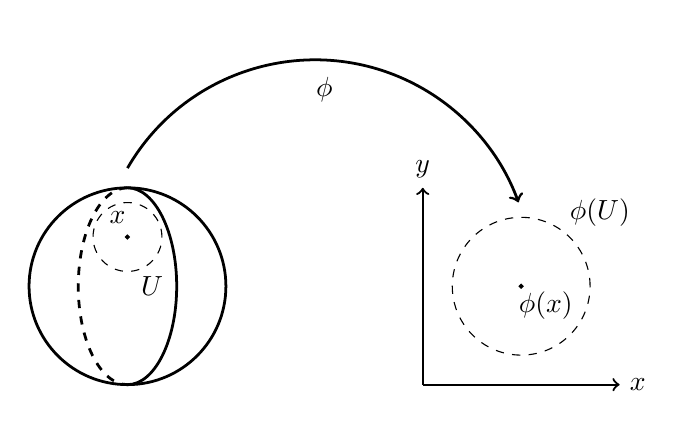
\begin{tikzpicture}[scale=1.25]
  \draw[line width=1] (-3,2) arc (90:-90:0.5 and 1);
  \draw[line width=1, dashed] (-3,2) arc (90:270:0.5 and 1);
  \draw[line width=1](-3,1) circle (1);
  \draw[color=black,thick,->] (0,0) -- (2,0) node[anchor=west]{$x$};
  \draw[color=black,thick,->] (0,0) -- (0,2) node[anchor=south]{$y$};

  \filldraw[black] (1,1) circle (0.02);
  \draw[dashed] (1,1) circle (0.7);
  \draw node at (1.25,0.80) {$\phi(x)$};
  \draw node at (1.8,1.75) {$\phi(U)$};

  \filldraw[black] (-3,1.5) circle (0.02);
  \draw node at (-3.1,1.70) {$x$};
  \draw[dashed] (-3,1.5) circle (0.35);
  \draw node at (-2.75,1) {$U$};

  \draw[line width=1, ->] (-3,2.2) arc (150:20:2.2);
  \draw node at (-1,3) {$\phi$};
\end{tikzpicture}

% 		\caption{Representación de un homeomorfismo de $\mathbb{S}^{2}$ a $\mathbb{R}^{2}$.}
% 	\end{figure}
% \end{frame}

\begin{frame}
	\frametitle{Ejemplo de variedades topológicas}
	\begin{columns}[t]
		\column{.5\textwidth}
		\centering
		\begin{figure}
			\scalebox{.5}{\tdplotsetmaincoords{70}{135}
\begin{tikzpicture}[scale=3,line join=bevel,tdplot_main_coords]
{\draw[color=black,thick,->] (0,0,0) -- (1,0,0) node[anchor=north east]{$x$};}%
{\draw[color=black,thick,->] (0,0,0) -- (0,1,0) node[anchor=north west]{$y$};}%
{\draw[color=black,thick,->] (0,0,0) -- (0,0,1) node[anchor=south]{$z$};}%
\end{tikzpicture}
}\\
			\caption{Los espacios euclidianos.}
		\end{figure}
		\begin{figure}
			\scalebox{.5}{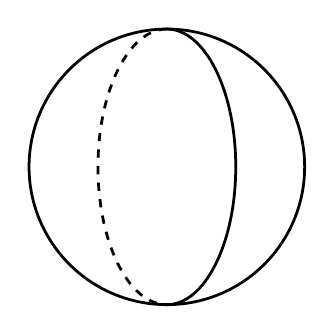
\begin{tikzpicture}[scale=1.75]
  \draw[line width=1] (0,1) arc (90:-90:0.5 and 1);
  \draw[line width=1, dashed] (0,1) arc (90:270:0.5 and 1);
  \draw[line width=1](0,0) circle (1);
\end{tikzpicture}
}\\
			\caption{Las $n-$Esferas.}
		\end{figure}
		\column{.5\textwidth}
		\centering
		\begin{figure}
			\vspace{12pt}
			\scalebox{.45}{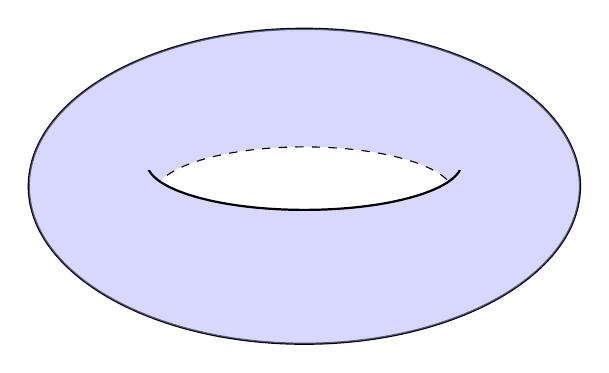
\begin{tikzpicture}[scale=2]
  % Elipse Principal
	\draw [thick] (0,0) ellipse  (1.75 and 1);
	\path[fill=blue!30!white,opacity=0.5] (0,0) ellipse  (1.75 and 1);

	%Arco inferior
	\begin{scope}
		\clip (0,0.15) ellipse (1 and 0.3);
		\fill[white] (0,-0.05) ellipse (0.95 and 0.3);
	\end{scope}

	% Arco superior
	\begin{scope}
		\clip (-1.25,0.03) rectangle (1.25,0.5);
		\draw[dashed] (0,-0.05) ellipse (0.95 and 0.3);
	\end{scope}

  % Centro
	\begin{scope}
		\clip (-1.25,0.1) rectangle (1.25,-0.5);
		\draw[thick] (0,0.15) ellipse (1 and 0.3);
	\end{scope}
\end{tikzpicture}
}\\
			\caption{Los $n-$Toros.}
		\end{figure}
		\begin{figure}
			\vspace{-6pt}
			\centering
			\scalebox{.55}{\begin{tikzpicture}[scale=4.5]
{\draw[color=black,thick,->] (0,0) -- (1,0) node[anchor=west]{$x$};}%
{\draw[color=black,thick,->] (0,0) -- (0,1) node[anchor=south]{$y$};}%
\draw[dashed] (0.5,0.5) circle (0.25);
\filldraw[black] (0.5,0.5) circle (0.02);
\end{tikzpicture}
}\\
			\caption{Los subconjuntos abiertos\\ de las variedades.}
		\end{figure}
	\end{columns}
\end{frame}

\begin{frame}
	\frametitle{Ejemplo: El espacio proyectivo}
	\centering
	\begin{figure}
		\scalebox{0.75}{\begin{tikzpicture}[scale=1.75]
\draw[color=black] (-2,0) -- (2,0);
\draw[color=black] (0,-2) -- (0,2);
\draw[thick] (0,0) circle (1);
\draw[thick] (-1.5, -1.5) -- (1.5,1.5); 
\filldraw[red] (0.71,0.71) circle (0.04);
\filldraw[blue] (-0.71,-0.71) circle (0.04);
\end{tikzpicture}
}
		\caption{Representación del espacio proyectivo $\mathbb{RP}^{1}$.}
		.\end{figure}
\end{frame}

\begin{frame}
	\frametitle{Cartas}
	\begin{definition}[Carta]
		Una \textbf{carta} en $M$ es un par ordenado $(U,\phi)$ donde $U$ es un subconjunto abierto de $M$ y $\phi$ es un homeomorfismo de $U$ a $\R^n$.
	\end{definition}\pause

	\begin{definition}[Cartas Suavemente Compatibles]
		Si $(U,\phi)$ y $(V,\psi)$ son dos cartas en $M$ tales que $U \cap V \neq \varnothing$, llamaremos \textbf{mapa de transición} a la composición de funciones:
		\[ \psi \circ \phi^{-1}: \phi(U \cap V) \to \psi(U \cap V) \]

		Diremos que las cartas $(U,\phi)$ y $(V,\psi)$ son \textbf{suavemente compatibles} si $U \cap V = \varnothing$ o si el mapa de transición $\psi \circ \phi^{-1}$ es un difeomorfismo.
	\end{definition}
\end{frame}

\begin{frame}
	\centering
	\begin{figure}
		\begin{tikzpicture}[scale=1]
	\coordinate (a) at (0,0);
	\path[draw,use Hobby shortcut,closed=true,thick]
	(0,2.5) .. (2,2.5) .. (1,4.5) .. (.3,4.5) .. (-1,4) .. (-2,2.5);

	\begin{scope}
		\clip (0.25,3.5) circle (0.5);
		\fill[blue!30!white,opacity=0.5] (-0.25,3.25) circle (0.5);
	\end{scope}
	\draw[dashed] (0.25,3.5) circle (0.5);
	\draw[dashed] (-0.25,3.25) circle (0.5);
	\draw node at (0.8,4) {$V$};
	\draw node at (-0.9,2.75) {$U$};

	\draw [thick, <->] (-5,0) -- (-1,0);
	\draw [thick, <->] (-3,-2) -- (-3,2);
	\draw [thick, <->] (1,0) -- (5,0);
	\draw [thick, <->] (3,-2) -- (3,2);

	\begin{scope}
		\clip (-3,0.5) ellipse  (0.8 and 1);
    \fill[color=blue!30!white,opacity=0.5] (-2.5,0) ellipse  (1.2 and 0.8);
	\end{scope}
	\draw [dashed,thick] (-3,0.5) ellipse  (0.8 and 1);
	% \draw [dashed,thick] (-2.5,0) ellipse  (1.2 and 0.8);

	\begin{scope}
		\clip (3,0.5) ellipse  (0.8 and 1);
		\fill[color=blue!30!white,opacity=0.5](3.5,0) ellipse  (1.2 and 0.8);
	\end{scope}
	% \draw [dashed,thick] (3,0.5) ellipse  (0.8 and 1);
	\draw [dashed,thick] (3.5,0) ellipse  (1.2 and 0.8);

	\draw[line width=1, ->] (1,3.75) arc (90:-5:2.5);
	\draw[line width=1, ->] (-1,3.25) arc (-90:0:-1.5);
	\draw[line width=1, ->] (-1.75,0.5) -- (2,0.5);

	\draw node at (-2.5,2.75) {$\phi$};
	\draw node at (3.25,3) {$\psi$};
	\draw node at (-4.25,1.25) {$\phi(U)$};
	\draw node at (4.5,1) {$\psi(V)$};
	\draw node at (0.25,1) {$\psi \circ \phi^{-1}$};


\end{tikzpicture}

		\caption{Mapa de transición}
	\end{figure}
\end{frame}


\begin{frame}
	\frametitle{Atlas y la estructura suave}
	\begin{definition}[Atlas, Atlas Suave y Atlas Maximal]
		\begin{itemize}
			\item Una colección de cartas $(U,\phi)_{\alpha}$ es un \textbf{atlas} $\mathcal{A}$, en $M$ si dichas cartas forman una cubierta para $M$.\pause
			\item Diremos que el atlas $\mathcal{A}$ es \textbf{suave} si cualesquiera dos cartas son suavemente compatibles, a las cartas de un atlas suave les llamaremos \textit{cartas suaves}.\pause
			\item Un atlas suave es llamado \textbf{maximal} si no está propiamente contenido en ningún atlas más grande.
		\end{itemize}
	\end{definition}

\end{frame}

\begin{frame}
	\centering
	\begin{figure}
		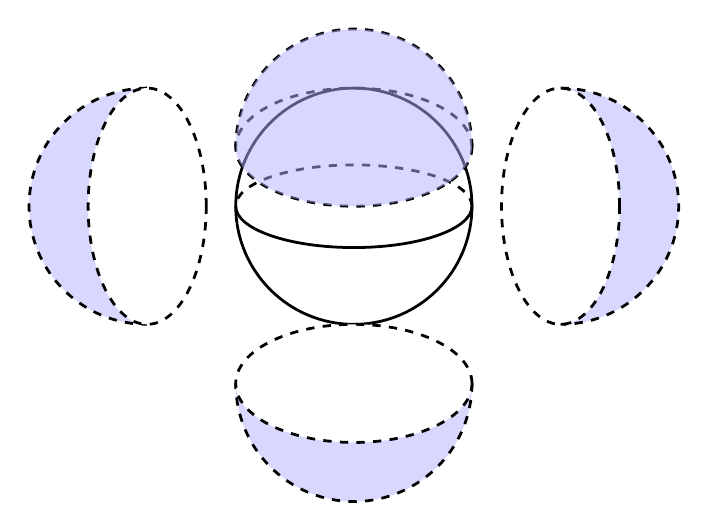
\begin{tikzpicture}[scale=1.5]
  \draw[line width=1, dashed] (1,0) arc (0:180:1 and 0.35);
  \draw[line width=1] (1,0) arc (0:180:1 and -0.35);
  \draw[line width=1](0,0) circle (1);

  % Left Chart
  \path[fill=blue!30!white,opacity=0.5] (-1.75,1) arc (90:-90:-1 and 1);
  \draw[line width=1, dashed] (-1.75,1) arc (90:-90:-1 and 1);
  \draw[fill=white, line width=1, dashed] (-1.75,0) ellipse (0.5 and 1);

  % Right Chart
  \path[fill=blue!30!white,opacity=0.5,line width=1, dashed] (1.75,1) arc (90:-90:1 and 1);
  \draw[fill=white, line width=1, dashed] (1.75,0) ellipse (0.5 and 1);
  \draw[line width=1, dashed] (1.75,1) arc (90:-90:1 and 1);

  % Top Chart
  \draw[line width=1, dashed] (0,0.5) ellipse (1 and 0.5);
  \draw[line width=1, dashed] (1,0.5) arc (0:180:1 and 1);
  \path[fill=blue!30!white,opacity=0.5] (1,0.5) arc (0:-180:1 and 0.5);
  \path[fill=blue!30!white,opacity=0.5] (1,0.5) arc (0:180:1 and 1);


  % Bottom Chart
  \path[fill=blue!30!white,opacity=0.5,line width=1, dashed] (1,-1.5) arc (0:-180:1 and 1);
  \draw[line width=1, dashed] (1,-1.5) arc (0:-180:1 and 1);
  \draw[fill=white, line width=1, dashed] (0,-1.5) ellipse (1 and 0.5);
\end{tikzpicture}

		\caption{Cuatro cartas suavemente compatibles en una esfera.}
	\end{figure}
\end{frame}

\begin{frame}
	\frametitle{Variedades Suaves}
	\begin{definition}[Variedad Suave]
		Si $M$ es una variedad topológica y $\mathcal{A}$ es un atlas maximal en $M$, diremos que el par $(M,\mathcal{A})$ es una \textbf{variedad suave}, a dicho atlas maximal le llamaremos la \textbf{estructura suave} en $M$.
	\end{definition}
\end{frame}

\begin{frame}
	\frametitle{Ejemplo de variedades suaves}
	\begin{columns}[t]
		\column{.5\textwidth}
		\centering
		\begin{figure}
			\scalebox{.5}{\tdplotsetmaincoords{70}{135}
\begin{tikzpicture}[scale=3,line join=bevel,tdplot_main_coords]
{\draw[color=black,thick,->] (0,0,0) -- (1,0,0) node[anchor=north east]{$x$};}%
{\draw[color=black,thick,->] (0,0,0) -- (0,1,0) node[anchor=north west]{$y$};}%
{\draw[color=black,thick,->] (0,0,0) -- (0,0,1) node[anchor=south]{$z$};}%
\end{tikzpicture}
}\\
			\caption{Los espacios euclidianos.}
		\end{figure}
		\begin{figure}
			\scalebox{.5}{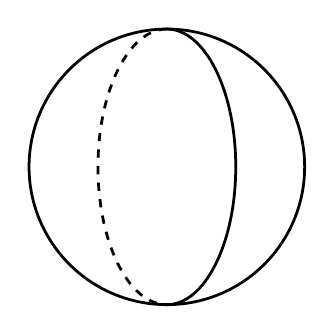
\begin{tikzpicture}[scale=1.75]
  \draw[line width=1] (0,1) arc (90:-90:0.5 and 1);
  \draw[line width=1, dashed] (0,1) arc (90:270:0.5 and 1);
  \draw[line width=1](0,0) circle (1);
\end{tikzpicture}
}\\
			\caption{Las $n-$Esferas.}
		\end{figure}
		\column{.5\textwidth}
		\centering
		\begin{figure}
			\vspace{12pt}
			\scalebox{.45}{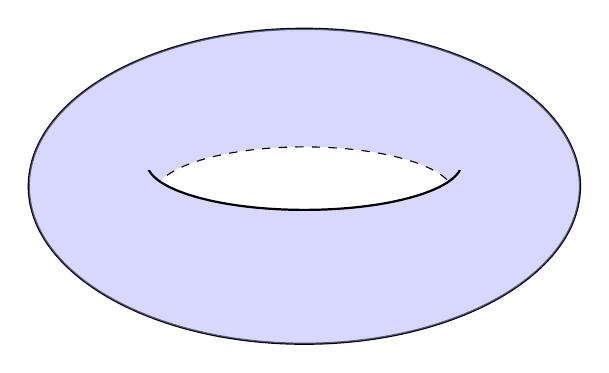
\begin{tikzpicture}[scale=2]
  % Elipse Principal
	\draw [thick] (0,0) ellipse  (1.75 and 1);
	\path[fill=blue!30!white,opacity=0.5] (0,0) ellipse  (1.75 and 1);

	%Arco inferior
	\begin{scope}
		\clip (0,0.15) ellipse (1 and 0.3);
		\fill[white] (0,-0.05) ellipse (0.95 and 0.3);
	\end{scope}

	% Arco superior
	\begin{scope}
		\clip (-1.25,0.03) rectangle (1.25,0.5);
		\draw[dashed] (0,-0.05) ellipse (0.95 and 0.3);
	\end{scope}

  % Centro
	\begin{scope}
		\clip (-1.25,0.1) rectangle (1.25,-0.5);
		\draw[thick] (0,0.15) ellipse (1 and 0.3);
	\end{scope}
\end{tikzpicture}
}\\
			\caption{Los $n-$Toro.}
		\end{figure}
		\begin{figure}
			\vspace{-6pt}
			\centering
			\scalebox{.55}{\begin{tikzpicture}[scale=4.5]
{\draw[color=black,thick,->] (0,0) -- (1,0) node[anchor=west]{$x$};}%
{\draw[color=black,thick,->] (0,0) -- (0,1) node[anchor=south]{$y$};}%
\draw[dashed] (0.5,0.5) circle (0.25);
\filldraw[black] (0.5,0.5) circle (0.02);
\end{tikzpicture}
}\\
			\caption{Los subconjuntos abiertos\\ de las variedades suaves.}
		\end{figure}
	\end{columns}
\end{frame}

\begin{frame}
	\frametitle{Funciones suaves}
	\begin{definition}[Función Suave]
		Sean $M$ una variedad suave  $n-$dimensional, $k$ un entero no negativo y $f: M \to \R^{k}$ una función. Diremos que $f$ es \textbf{suave} si para cada punto $p \in M$ existe una carta suave $(U,\phi)$, cuyo dominio contiene a $p$, tal que la composición de funciones $f \circ \phi^{-1}$ es suave en $\phi(U) \subseteq \R^{n}$.
	\end{definition}
	\begin{figure}
		\scalebox{0.6}{\begin{tikzpicture}[scale=0.85]
  \coordinate (a) at (0,0);
\path[draw,use Hobby shortcut,closed=true,thick]
(0,2.5) .. (2,2.5) .. (1,4.5) .. (.3,4.5) .. (-1,4) .. (-2,2.5);

\draw[dashed] (0.25,3.5) circle (0.6);
\draw node at (0,3.6) {$U$};
\draw node at (-1.5,4.5) {$M$};

\draw [thick, <->] (-5,0) -- (-1,0);
\draw [thick, <->] (-3,-2) -- (-3,2);
\draw [thick, <->] (1,0) -- (5,0);
\draw [thick, <->] (3,-2) -- (3,2);

\draw [dashed,thick] (-3,-0.25) ellipse  (1.5 and 1.2);


\draw[line width=1, ->] (1,3.75) arc (90:0:2.5);
\draw[line width=1, ->] (-0.75,3.5) arc (-90:0:-2);
\draw[line width=1, ->] (-1.5,-1.5) arc (60:120:-3.5);

\draw node at (-2.75,3) {$\phi$};
\draw node at (3.25,3) {$f$};
\draw node at (-2.25,-0.5) {$\phi(U)$};
\draw node at (-4.5,1) {$\R^n$};
\draw node at (4.5,1) {$\R^{k}$};
\draw node at (0.5,-1.25) {$f \circ \phi^{-1}$};
\end{tikzpicture}
}
		\caption{Representación de una función suave.}
	\end{figure}
\end{frame}

\begin{frame}
	\begin{figure}
		\scalebox{.70}{\begin{tikzpicture}[scale=1]

%Variedad M
\path[draw,use Hobby shortcut,closed=true]
(-5,5.5) .. (-6,4) .. (-4,4) .. (-2,3.5) .. (-2.5,6);
\filldraw (-3,5) circle (0.05);
\node at (-3.25,5.25) {$p$};
\node at (-2.25,4.35) {$U$};
\draw[dashed] (-3,5) ellipse (0.6 and 0.8);
\node at (-1.25,5.75) {$M$};

%Variedad N
\path[draw,use Hobby shortcut,closed=true]
(5.5,6) .. (6,4) .. (4,3) .. (2,3.5) .. (2.5,5) .. (3.5,5.5);
\filldraw (3.25,4) circle (0.05);
\node at (2.75,3.6) {$F(p)$};
\node at (4.25,5) {$V$};
\draw[dashed](3.25,4) ellipse (1.2 and 0.9);
\node at (2,5.25) {$N$};

% Flecha M a N
\draw[thick,->] (-1,6) arc (-60:-130:-2.5);
\node at (0.25,6.75) {$F$};

% Flecha M a Rm
\draw[thick,->] (-3,4) arc (-10:20:-5);
\node at (-3.5,2.75) {$\phi$};

% Flecha N a Rn
\draw[thick,->] (3.75,3.25) arc (10:-20:4);
\node at (4.25,2) {$\psi$};

%Eje Izquierdo
\draw [<->] (-5,-1) -- (-1,-1);
\draw [<->] (-4,-1.5) -- (-4,2.5);
\node at (-5,2.5) {$\R^m$};
\node at (-1,1.25) {$\phi(U)$};
\draw[dashed] (-2.5, 0.25) circle (1);

%Eje Derecho
\draw [<->] (5,-1) -- (1,-1);
\draw [<->] (2,-1.5) -- (2,2.5);
\node at (1,2.5) {$\R^n$};
\node at (4.5,0) {$\psi(V)$};
\draw[dashed] (2.5, -0.25) circle (1.2);

% Flecha Rn a Rm
\draw[thick,->] (-2,-1.25) arc (60:120:-3.5);
\node at (0,-2) {$\psi \circ F \circ \phi^{-1}$};
\end{tikzpicture}
}
		\caption{Representación de un mapa suave.}
	\end{figure}
\end{frame}

\begin{frame}
	\frametitle{Ejemplo de funciones y mapas suaves}
	\begin{itemize}
		\item El mapa identidad.
		\item El mapa de inclusión
		\item Los mapas constantes.
		\item Las proyecciones.
		\item La composición de funciones suaves.
	\end{itemize}
\end{frame}

\begin{frame}
\frametitle{Espacios Tangentes en $\R^n$}
\begin{definition}[Vectores y Espacios Tangentes en $\R^n$]\label{Definición: Espacio Tangente en Rn}
Sea $a$ un punto en $\R^n$, definiremos el \textbf{espacio tangente a $\R^n$ en el punto $a$}, denotado por $T_a(\R^n)$, como el conjunto:
  \[ \{a\} \times \R^n = \{(a,v): v \in \R^n\} \]
  
  Un \bf{vector tangente} a $\R^n$ es un elemento de $T_a(\R^n)$ para algún $a \in \R^n$. Denotaremos a un vector tangente $(a,v)$ particular como $v_a$ o simplemente $v$ para abreviar.
\end{definition}\pause

  Una de las propiedades más importantes del conjunto $T_a(\R^n)$ es que tiene estructura de espacio vectorial bajo las operaciones
  \[v_a + w_a = (v+w)_a, \quad c(v_a) = (cv)_a\]
  Además, este espacio vectorial es isomorfo a $\R^n$.
\end{frame}

\begin{frame}
\begin{columns}[t]
\column{.5\textwidth}
\centering
  \begin{figure}
    \centering
    \scalebox{0.75}{\input{./Figuras/EspacioTangente.tex}}
    \caption{Representación del espacio \\ tangente $T_a(\R^n)$.}
  \end{figure}
\column{.5\textwidth}
\centering
  \begin{figure}
    \centering
    \scalebox{0.65}{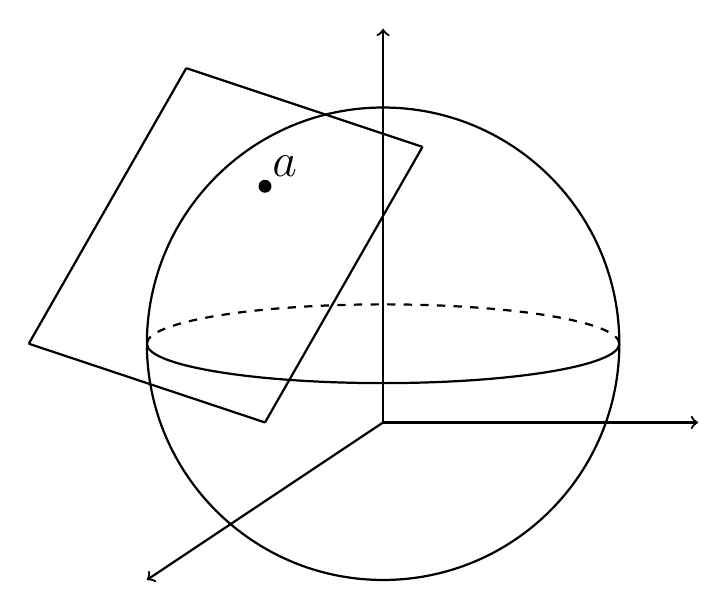
\begin{tikzpicture}
  % Esfera
  \draw [thick] (3,0) arc (0:180:3 and -0.5);
  \draw [thick, dashed] (-3,0) arc (180:0:3 and 0.5);
  \draw [thick] (0,0) circle (3);

  % Ejes R3
  \draw [thick,->] (0,-1) -- (0,4);
  \draw [thick,->] (0,-1) -- (4,-1);
  \draw [thick,->] (0,-1) -- (-3,-3);


  % Rectángulo (Espacio Tangente)
  \filldraw (-1.5,2) circle (0.075);
  \node[font=\fontsize{18pt}{18pt}] at (-1.25,2.25) {$a$};
  \draw [thick] (-2.5,3.5) -- (0.5,2.5);
  \draw [thick] (-2.5,3.5) -- (-4.5,0);
  \draw [thick] (-4.5,0) -- (-1.5,-1);
  \draw [thick] (0.5,2.5) -- (-1.5,-1);
\end{tikzpicture}
}
    \caption{Representación del espacio \\ tangente a una esfera.}
  \end{figure}
\end{columns}
\end{frame}

\begin{frame}
  Si tenemos un punto $a = (a_1, \dots, a_n) \in \R^n$ y un vector $\begin{bmatrix} v_1 \dots v_n \end{bmatrix}$ podemos parametrizar la recta que pasa por $a$ con dirección $v$ de la siguiente manera:

  \[\gamma(t) = a_1 + tv_1, \dots, a_n + tv_n \]
  \pause
  Teniendo esto en cuenta, y, por nuestros cursos de cálculo sabemos que si $f: \R^n \to \R$ es una función suave definida en un punto $a$ y $v \in T_a(\R^n)$ podemos obtener la derivada direccional de $f$ en $a$ en la dirección de $v$ como:
  \[
    D_v f = \left. \frac{d}{dt}\right|_{t=0} f(\gamma(t)) 
    = \sum_{i=1}^{n} v_i \left. \frac{\partial f}{\partial x_i} \right|_{a}
  \]
\end{frame}

\begin{frame}
  Hay dos propiedades que nos interesan particularmente de la derivada direccional. La derivada direccional es lineal y cumple la regla de Leibniz. Esto quiere decir que si $f$ y $g$ son funciones suaves definida en una vecindad de $a \in \R^n$, $c$ es una constante y $v \in T_{a}(\R^n)$, entonces:

  \begin{itemize}
    \item $D_v(f+g) = D_v(f) + D_v(g)$
    \item $D_v(cf) = cD_v(f)$
    \item $D_v(fg) = f(a)D_v(g) + g(a)D_v(f)$ 
  \end{itemize}
\end{frame}

\begin{frame}
  Basándonos en las propiedades anteriores de las derivaciones es que se darán las siguientes definiciones.
  \begin{definition}[Derivación en un punto]
    Si $a$ es un punto en $\R^n$ y $\omega: C^{\infty}(\R^{n}) \to \R$ es un funcional lineal, diremos que $\omega$ es una \textbf{derivación} en $a$ si cumple la regla de Leibniz. Esto es, si $f$ y $g$ son funciones suaves definidas en una vecindad de $a$ y $c$ es una constante, entonces:
    \begin{itemize}
      \item $\omega(cf) = c \omega(f)$
      \item $\omega(f+g) = \omega(f) + \omega(g)$
      \item $\omega(fg) = f(a)\omega(g) + g(a)\omega(f)$
    \end{itemize}
  \end{definition}

\end{frame}

\begin{frame}
  El conjunto de todas las derivaciones en $a$, el cual denotamos por $\mathcal{D}_a(\R^n)$ es, curiosamente, un espacio vectorial bajo las operaciones:
  \begin{align*}
    (\omega_1 + \omega_2)(f) &= \omega_1(f) + \omega_2(f)\\
    (c\omega)(f) &= c(\omega(f))
  \end{align*} \pause

  Y quizá todavía más curioso es el siguiente teorema:
\end{frame}

\begin{frame}
\begin{theorem}
  Los espacios $T_a(\R^n) \to \mathcal{D}_a(\R^n)$ son isomorfos y el isomorfismo de espacios vectoriales está dado por:
\begin{align*}
  \phi: T_a(\R^n) &\to \mathcal{D}_a(\R^n)\\
  v &\mapsto D_v = \sum_{i=1}^n v_i \left. \frac{\partial}{\partial x_i} \right|_{a}
\end{align*}
\end{theorem}\pause

  Dos consecuencias de este teorema es que el espacio de derivaciones en un punto $a$, $\mathcal{D}_a(\R^n)$ es isomorfo a $\R^n$ y que para cada $a \in \R^n$, las $n$ derivadas parciales:
  \[
    \left. \frac{\partial}{\partial x_1} \right|_a,
    \dots,
    \left. \frac{\partial}{\partial x_n} \right|_a
  \]
  forman una base para el espacio tangente $T_a(\R^n)$
\end{frame}

\begin{frame}
\begin{definition}[Derivación en un punto de una variedad]
  Sea $M$ una variedad suave y sea $p \in M$ un punto. Diremos que en mapa $\omega: C^{\infty}(M) \to \R$ es una \textbf{derivación} en $p$ si es lineal y además cumple la regla de Leibniz.

  Llamaremos al conjunto de todas las derivaciones en un punto de una variedad el \textbf{espacio tangente} a la variedad en ese punto, y denotaremos al conjunto por $T_p(M)$.
\end{definition}\pause

  El espacio tangente $T_p(M)$ también es un espacio vectorial bajo operaciones idénticas a las vistas anteriormente.
\end{frame}

\begin{frame}
  Ahora quisiéramos estudiar como es que los mapas suaves entre variedades afectan a los vectores del espacio tangente.

  \begin{definition}[Diferencial de un mapa]
    Si $M$ y $N$ son variedades suaves y $F: M \to N$ es un mapa suave, entonces para cada punto $p \in M$ el mapa $F$ induce un mapeo lineal entre $T_p(M)$ y $T_{F(p)}(N)$, denotado $dF_p: T_p(M) \to T_{F(p)}(N)$, a este mapa le llamamos el \textbf{diferencial de F en p}.

    El mapa $dF_p$ está dado por: Dada un vector tangente $\omega \in T_p(M)$, $dF_p$ será la derivación en el punto $F(p) \in N$ que actúa sobre funciones suaves $f: N \to \R$ del siguiente modo:
    \[
      dF_p(\omega)(f) = \omega(f \circ F)
    \]
  \end{definition}
\end{frame}

\begin{frame}
  \begin{figure}
    \centering
    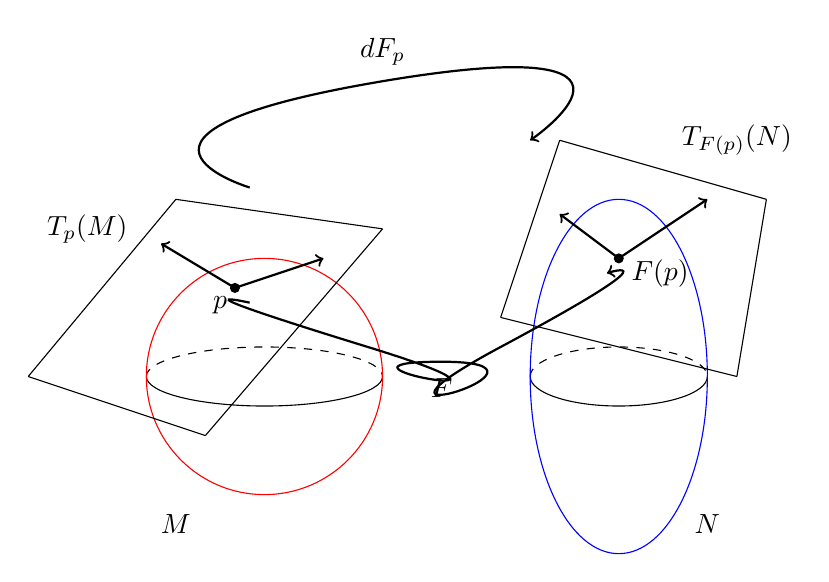
\begin{tikzpicture}[scale=0.75]
  % Esfera
  \draw (-4,0) arc (0:180:2 and -0.5);
  \draw [dashed] (-8,0) arc (180:0:2 and 0.5);
  \draw [red] (-6,0) circle (2);
  \node at (-7.5,-2.5) {$M$};
  \node at (-6.75,1.2) {$p$};
  \node at (-9,2.5) {$T_p(M)$};

  % Rectángulo (Espacio Tangente a Esfera)
  \filldraw (-6.5,1.5) circle (0.075);
  \draw[thick,->] (-6.5,1.5) -- (-5,2);
  \draw[thick,->] (-6.5,1.5) -- (-7.75,2.25);
  \draw  (-7.5,3) -- (-4,2.5);
  \draw  (-4,2.5) -- (-7,-1);
  \draw  (-7,-1) -- (-10,0);
  \draw  (-10,0) -- (-7.5,3);

  % Elipsoide
  \draw (1.5,0) arc (0:180:1.5 and -0.5);
  \draw [dashed] (-1.5,0) arc (180:0:1.5 and 0.5);
  \draw [blue] (0,0) ellipse (1.5 and 3);
  \node at (1.5,-2.5) {$N$};
  \node at (0.7,1.75) {$F(p)$};
  \node at (2,4) {$T_{F(p)}(N)$};

  % Rectángulo (Espacio Tangente a Elipsoide)
  \filldraw (0,2) circle (0.075);
  \draw[thick,->] (0,2) -- (1.5,3);
  \draw[thick,->] (0,2) -- (-1,2.75);
  \draw (-2,1) -- (2,0);
  \draw (2,0) -- (2.5,3);
  \draw (2.5,3) -- (-1,4);
  \draw (-1,4) -- (-2,1);

  % Flechas
  \draw[thick, ->] plot [smooth,tension=4] coordinates {(-6.25,1.25) (-4.25,0.5) (-3,0.25) (-2,0.5) (-0.20,1.75)};
  \node at (-3,-0.20) {$F$};
  \draw[thick, ->] plot [smooth,tension=4] coordinates {(-6.25,3.2) (-4,5) (-1.5,4)};
  \node at (-4,5.5) {$dF_p$};

\end{tikzpicture}

    \caption{Representación del diferencial de un mapa}
  \end{figure}
\end{frame}

\begin{frame}
  Los espacios tangentes son muy útiles, sin embargo, para nuestros fines será necesario ser capaces de considerar más de un espacio tangente a la vez, esto se puede hacer considerando el fibrado tangente.
  
\begin{definition}[Fibrado Tangente]
  Dada una variedad suave $M$, definimos el \textbf{fibrado tangente de $M$}, el cual denotaremos por $TM$, como la unión disjunta de todos los espacios tangentes a $M$:
\[ TM = \bigsqcup_{p \in M} T_p(M) = \bigcup_{p \in M} \{p\} \times T_p(M) \]
\end{definition}
\end{frame}

\begin{frame}
  \centering
  \begin{figure}
  \includegraphics[width=0.8\textwidth]{./Figuras/TangentBundle.png}
    \caption{Espacios Tangentes y Fibrado Tangente de $\S^{1}$.}
  \end{figure}
\end{frame}

\begin{frame}
  \begin{theorem}
    Sea $M^n$ una variedad suave, el fibrado tangente $TM$ tiene una topología natural y una estructura suave que vuelven a $TM$ una variedad suave $2n-$dimensional de tal modo que la proyección $\pi: TM \to M$ es suave con respecto a dicha estructura suave.
  \end{theorem}
\end{frame}



\begin{frame}
\begin{definition}[Campo Vectorial]
  Un \textbf{campo vectorial} $X$ en una variedad $M$ es una sección del fibrado tangente $\pi: TM \to M$, esto es, $X: M \to TM$ es un mapa tal que $X(p) \in T_{p}(M)$ para cada $p \in M$. Además diremos que que es un \textbf{campo vectorial suave} si $X$ es un mapa suave. Denotaremos al conjunto formado por todas los campos vectoriales suaves en $M$ como $\mathfrak{X}(M)$
\end{definition}
\end{frame}

\begin{frame}
  \centering
  \begin{figure}
  \includegraphics[width=0.8\textwidth]{./Figuras/CampoVectorial.png}
    \caption{Representación de un campo vectorial.}
  \end{figure}
\end{frame}

\input{Contenido/06-Metricas.tex}

\end{document}

